\documentclass[10pt,review,sigplan,anonymous=true]{acmart}
\settopmatter{printfolios=false,printccs=false,printacmref=false}

\bibliographystyle{ACM-Reference-Format}
\citestyle{acmauthoryear}   %% For author/year citations
\usepackage{listings,multirow,wrapfig,xspace,paralist}
\usepackage{xcolor,tikz,graphicx, pifont}
%\usetikzlibrary{positioning}

%% \newcommand{\authorcomment}[3]{\xspace\textcolor{#1}{{\bf #2} #3}\xspace}
\newcommand{\authorcomment}[3]{}
% For author notes:
\newcommand{\AG}[1]{\authorcomment{orange}{AG}{#1}}
\newcommand{\JV}[1]{\authorcomment{red}{JV}{#1}}

% For meta comments:
\newcommand{\isit}[1]{\authorcomment{cyan}{Check}{#1}}
\newcommand{\todo}[1]{\authorcomment{red}{TODO}{#1}}
\newcommand{\xmark}{\textcolor{red}{\ding{55}}}
\newcommand{\cmark}{\textcolor{green}{\ding{51}}}

\definecolor{LightGray}{RGB}{247, 247, 247}
\definecolor{Gray}{rgb}{.3,.3,.3}
\definecolor{DarkGray}{rgb}{.5,.5,.5}

%% https://www.davehofmann.de/defining-custom-language-templates-for-latex-listings/
% Define Language
\lstdefinelanguage{smalleR} {
  % list of keywords
  morekeywords={
    for,
    if,
    else,
    function
  },
  sensitive=true, % keywords are not case-sensitive
  morecomment=[l]{\#}, % l is for line comment
  morestring=[b]{"} % defines that strings are enclosed in double quotes
}

\lstset{
  language={smalleR},
  columns=flexible,
  captionpos=b,
  frame=single,
  framerule=0pt,
  framexleftmargin=1mm,
  framexrightmargin=1mm,
  tabsize=2,
  belowskip=0pt,
  basicstyle=\small\ttfamily,
  backgroundcolor=\color{LightGray},
  emphstyle=\sffamily,
  keywordstyle=\bfseries,
  commentstyle=\color{Gray}\em,
  stringstyle=\color{Gray},
  alsoletter={., _, $},
  breaklines=true
}

\newcommand{\code}[1]{\lstinline |#1|\xspace}
\renewcommand{\c}[1]{\lstinline |#1|\xspace}
\newcommand{\eg}{\emph{e.g.},\xspace}
\newcommand{\ie}{\emph{i.e.},\xspace}

\newcommand{\environmentFun}{\code{environment}}

\newcommand{\emptyenv}{\code{empyenv}}
\newcommand{\globalenv}{\code{globalenv}}

\newcommand{\newEnv}{\code{new.env}}

\newcommand{\asList}{\code{as.list}}
\newcommand{\listToEnv}{\code{list2env}}

\newcommand{\ls}{\code{ls}}
\newcommand{\objects}{\code{objects}}

\newcommand{\subDollar}{\code{$}}
\newcommand{\subBracket}{\code{[[}}

\newcommand{\exist}{\code{exist}}

\newcommand{\get}{\code{get}}
\newcommand{\getZero}{\code{get0}}
\newcommand{\mget}{\code{mget}}
\newcommand{\dynGet}{\code{dynGet}}

\newcommand{\assign}{\code{assign}}

\newcommand{\remove}{\code{remove}}
\renewcommand{\rm}{\code{rm}}

\newcommand{\parentEnv}{\code{parent.env}}
\newcommand{\parentEnvAssign}{\code{parent.env<-}}

\newcommand{\envtracer}{\texttt{envtracer}\xspace}
\newcommand{\experimentr}{\texttt{experimentr}\xspace}

\newcommand{\ggplot}{\textit{ggplot2}\xspace}
\newcommand{\vctrs}{\textit{vctrs}\xspace}

%%% \setcopyright{rightsretained}
%%% \acmPrice{}
%%% \acmDOI{10.1145/3360579}
%%% \acmYear{2019}
%%% \copyrightyear{2019}
%%% \acmJournal{PACMPL}
%%% \acmVolume{3}
%%% \acmNumber{OOPSLA}
%% \acmArticle{153}
%%% \acmMonth{10}
\begin{document}
\title{On the Use of First-Class Environments in R}

\author{Aviral Goel}\affiliation{\institution{Northeastern University}\country{USA}}
\author{Jan Vitek}\affiliation{\institution{Czech Technical University and Northeastern University}\country{USA}}
\authorsaddresses{}
\renewcommand{\shortauthors}{Goel, et al.}


\begin{abstract}
  The R programming language is widely used for statistical computations. R
  encourages a very dynamic programming style, to enable interactive data
  exploration and rapid prototyping. A key enabler of this dynamism is its
  support for first-class environments. To our knowledge, R is the only
  mainstream programming language with explicit environments. This paper
  presents the design of environments in R, and an empirical evaluation of how
  they are used. For this, we analyze \AG{XXXX} programs from 100 most popular CRAN
  packages. We find that first-class environments are used for \AG{XYZ}.
\end{abstract}

\begin{CCSXML}
<ccs2012>
<concept>
<concept_id>10002944.10011123.10010912</concept_id>
<concept_desc>General and reference~Empirical studies</concept_desc>
<concept_significance>500</concept_significance>
</concept>
<concept>
<concept_id>10011007.10011006.10011008</concept_id>
<concept_desc>Software and its engineering~General programming languages</concept_desc>
<concept_significance>500</concept_significance>
</concept>
<concept>
<concept_id>10011007.10011006.10011050.10010517</concept_id>
<concept_desc>Software and its engineering~Scripting languages</concept_desc>
<concept_significance>500</concept_significance>
</concept>
<concept>
<concept_id>10011007.10011006.10011039.10011311</concept_id>
<concept_desc>Software and its engineering~Semantics</concept_desc>
<concept_significance>300</concept_significance>
</concept>
</ccs2012>
\end{CCSXML}

\ccsdesc[500]{General and reference~Empirical studies}
\ccsdesc[500]{Software and its engineering~General programming languages}
\ccsdesc[500]{Software and its engineering~Scripting languages}
\ccsdesc[300]{Software and its engineering~Semantics}

%\keywords{R language, delayed or lazy evaluation}

\maketitle
\section{Introduction}

{\small \medskip\noindent\emph{Availability.} Our work is in open source, experiments are
repeatable and will be submitted to the AEC.}

\section{Background}\label{sec:background}

\subsection{Related Work}
%- \code{https://picolisp.com/wiki/?firstclassenvironments}
%- \code{http://metamodular.com/SICL/environments.pdf}
%- \code{Free variables and first-class environments}
%% https://link.springer.com/article/10.1007%2FBF01813016
%-
%\code{https://groups.csail.mit.edu/mac/ftpdir/scheme-7.4/doc-html/scheme_14.html}
%- \code{Environments as First Class Objects}
%- \code{Explicit Environments}
%% https://link.springer.com/chapter/10.1007%2F3-540-48959-2_24
%- \code{Simply Typed Lambda Calculus with First-Class Environments}
%% https://www.ems-ph.org/journals/show_abstract.php?issn=0034-5318&vol=30&iss=6&rank=4
%- \code{ML with first-class environments and its type inference algorithm}
%% https://link.springer.com/chapter/10.1007%2FBFb0032396
%- \code{https://adv-r.hadley.nz/environments.html}
%- \code{Sharing Code through First-class Environments}
%% https://pages.lip6.fr/Christian.Queinnec/PDF/modenv.pdf
%- \code{Environments as first class objects}
%% https://dl.acm.org/doi/10.1145/41625.41634
%Python locals vs globals
%%(https://realpython.com/python-namespaces-scope/#the-local-and-enclosing-namespaces)
%- Scheme R5RS standard talks about environment for two argument eval.


\subsection{The R Language}

R is a vectorized, dynamic, lazy, functional and object-oriented programming
language, designed by Ihaka and Gentleman in 1993 as a successor to S. In this
section, we provide a brief primer on R, with a focus on environments.

R has first-class, anonymous, lexically scoped functions. They are the most
important linguistic construct; all expressions (bracketing, operators, etc.)
desugar to function calls.

Vectors in R are homogeneous fixed-size arrays of integer, double, character
(string), logical (boolean), complex, or raw (byte) values. Lists are
heterogeneous vectors with optionally named elements. They can be indexed by
position or name. R objects can be tagged with user-defined data called
attributes. They are an optional name value map typically used to add a
domain-specific type structure. For example, \code{attr(x, dim) <- c(2, 2))}
attaches the attribute \code{dim} to vector \code{x <- c(1,2,3,4)} and R
subsequently treats it as a 2$\times$2 matrix. Of special interest is the
\code{class} attribute. \code{class(x) <- c("cat", "animal")} sets the class of
\code{x} to \code{"cat"} and \code{"animal"}. This is used for object-oriented
programming by S3 and S4, two OOP frameworks of R. S3 uses the \code{class}
attribute to dispatch on the first argument, and S4 allows multiple dispatch.
Formula is a compact symbolic representation of models used by model fitting
functions. For example, the linear model \code{y ~ x - 1} specifies a line
through the origin. Formula contains a reference to the environment in which it
is defined to refer to the variables, if they are not otherwise provided during
model fitting.

Environments bind (unique) names to values. They are backed either by an
association list (default) or a hash table, chosen on initialization. Unlike
other R objects, they are modified by reference. Environments form a chain; each
environment points to a parent environment. The chain terminates at the
\code{empty} environment; which is always empty. The call, \code{emptyenv()},
returns the \code{empty} environment.

\subsubsection{Environments as Packages}

Packages loaded by calling \code{library} are represented as environments; their
names are added to a global search path (returned by \code{search()}) for
lookup. The \code{n}th package environment can be retrieved using
\code{pos.to.env(n)}. Each package has a corresponding namespace environment
which also contains its private bindings and implementation specific metadata.
The namespace environment for a package named \code{ns} can be obtained by
\code{asNamespace(ns)}. An R session starts with the \code{base} package
preloaded, which contains the default R APIs. \code{baseenv()} returns the
\code{base} package environment and \code{.BaseNamespaceEnv} is bound to the
\code{base} package namespace.

\subsubsection{Environments as Scopes}
The top-level scope is the \code{global} environment, referred by the variable
\code{.GlobalEnv}, or returned by \code{globalenv()}. The \code{environment()}
call returns the current evaluation environment. At the top level, it returns
the \code{global} environment, and inside a function, it returns the function's
environment. When supplied with a function argument, it returns the function's
definition environment. \code{environment(fun) <- env} sets \code{env} as the
environment of \code{fun}.

\begin{lstlisting}
> f <- function() { print(environment()) }
> environment(); environment(f); f()
<env: Global> <env: Global> <env: 0x7ff>
> e <- new.env(); print(e)
<env: 0x7f1>
> environment(f) <- e; environment(f)
<env: 0x7f1>
\end{lstlisting}

R provides a rich call stack reflection interface, which can be divided into two
categories. The first category provides the frame numbers. Frame number starts
from 0, for \code{global} environment (top level), and increases by 1 for each
nested call. \code{sys.nframe()} returns the current frame number.
\code{sys.parent(n)} returns the frame number of the \code{n}th parent (caller
if \code{n} is 1). The second set yields a frame's environment.
\code{sys.frame(which)} returns the environment of the frame at position
\code{which} (counting backwards if \code{which} is negative).
\code{parent.frame(n)} is an optimized implementation of
\code{sys.frame(sys.parent(n))}. Lastly, \code{sys.frames()} returns a list of
all active frames' environments.

\begin{lstlisting}
> f <- function() { print(environment())
>     g <- function() { parent.frame(1) }; g() }
> f()
<env: 0x7f2> <env: 0x7f2>
\end{lstlisting}

\subsubsection{Environments as Data Structures}
Environments can be created using the \newEnv function. This function takes
three arguments: \code{hash}, a boolean for selecting a hash table
representation over the default association list representation, \code{size}, a
number specifying the size for preallocation, and, \code{parent}, the enclosing
environment. R does not provide any function to query the representation used
for an environment.The \code{length} function of an environment (number of
bindings) can be obtained using the. \parentEnv yields the enclosing environment
of an environment and \code{parent.env(envir) <- parent} sets the enclosing
environment of \code{envir} to \code{parent}.

\begin{lstlisting}
> e <- new.env(parent=emptyenv()); length(e)
0
> parent.env(e)
<environment: R_EmptyEnv>
> parent.env(e) <- globalenv(); parent.env(e)
<environment: R_GlobalEnv>
\end{lstlisting}

\asList converts environments to lists, heterogeneous vectors with optionally
named elements. \listToEnv copies the elements of a list to an environment. If
the environment is not supplied, it creates one using \newEnv. The variables of
an environment can be retrieved as a vector using the \ls and \objects
functions.

\begin{lstlisting}
> l <- list(x=1, y=2); e <- list2env(l); length(e)
2
> as.list(e)
list(y = 2, x = 1)
> ls(e)
[1] "x" "y"
\end{lstlisting}

A variable's existence in an environment can be queried using \exist. Its value
can be retrieved using \subDollar and \subBracket operators. \get, \getZero,
\mget, and \dynGet functions are generalizations of these operators with options
to perform lookup recursively in parent environments (\code{inherits = TRUE})
and validate the type of value bound to the variable being read (\code{mode =
  "integer"}). \getZero is \get with an extra argument, \code{ifnotfound}, which
is returned if the variable is not present in the environment. \mget is a
vectorized version of \get; it reads multiples variables supplied as a vector
and returns a vector of values. \dynGet performs recursive lookups in caller
frames, i.e., dynamic scopes, unlike the other functions which perform lookup in
lexical scopes.

\textit{Writes.} Writes can be performed using the \assign function. Variables
can be removed using the \rm and \remove function.

TODO - eval and environment.

\paragraph{Discussion.} R provides a vast API for accessing scopes as reified
environments and interacting with them. This makes them very versatile objects.
While they primarily serve as scopes, they can also be used as hash tables, and
sandboxing expression evaluation. While R is lexically scoped, ad-hoc lookup
strategies can be implemented by accessing arbitrary caller environments. The
lexical scope of a function can be changed, a technique often used for designing
custom object-oriented systems.

\section{Analysis Infrastructure}
In this section, we describe the tracing infrastructure and the data analysis
pipeline used for this study. The tracing infrastructure mainly consists of a
modified R VM, which raises events during a program's execution. These events
are processed to collect execution traces which are analyzed offline.
The analysis pipeline assembles the corpus, runs the tracer, and ...

The analysis pipeline has three main steps. First, the scripts assemble
the corpus. In this step, we download and install R packages from CRAN, and
extract executable programs from them. Second, we

- corpus
- run
- data nalysis
- manaaged by a makefile

\section{Corpus of R Programs}

For this study, we assembled a corpus of 100 most widely used packages from
CRAN, based on the number of client packages. These packages together have
11,786 clients. Package \ggplot has the highest number of clients, 2,320, and
package \vctrs has the fewest, 108. These packages contribute 481.5K lines of R
code and 1M lines of native code. During execution, these 100 packages call
functions from 186 other packages, so our evaluation also includes them. These extra
packages have 478.2K lines of R code and 1.1M lines of native code.


\begin{table}[!h]
  \vspace{-3mm}
  \small
  \centering
  \caption{Corpus}\label{table:corpus}
  \vspace{-3mm}
  \begin{tabular}{lrrr}
    \toprule
    &\bf Tests&\bf Examples&\bf Vignettes\\
    \midrule
    {Scripts}&1.9K&5.0K&187.0\\
    \midrule
    {LOC}&136.7K&55.2K&13.9K\\
    \bottomrule
  \end{tabular}
\end{table}

CRAN packages come equipped with runnable code in the form of tests, examples,
and long-form examples called vignettes. These programs are extracted as
independently executable scripts for evaluation by the \experimentr library.
Experiments demonstrate the use of a package's functions, and vignettes
illustrate a package's functionality with a larger example, typically using data
supplied with the package. Table~\ref{table:corpus} presents the number and size
of these scripts. Overall, there are 6.1K scripts with 205.8K lines of code.

The 286 corpus packages have 44.3K top-level functions, of which, 18.7K
functions are exercised by the extracted scripts. From the un-exercised 25.6K
functions, the majority, 17.2K, belong to transitively included packages, and,
8.4K belong to the initially selected 100 packages. Since the executable scripts
are extracted from 100 packages, they don't provide good coverage for the
transitively included 186 packages.

Table~\ref{table:fundist} presents the distribution of exercised functions
across these packages. We observe that 171 packages have 25 functions or less.
There are few large packages; 8 packages have more than 500 functions.

\begin{table}[!h]
  \vspace{-2mm}
  \small
  \caption{Package Size} \label{table:packsize}
  \centering
  \begin{tabular}{lr}
    \toprule
    \bf Functions&\bf Packages\\
    \midrule
    1--25&169\\
    26--50&40\\
    51--100&17\\
    101--150&14\\
    151--200&11\\
    201--250&15\\
    \bottomrule
  \end{tabular}
  \quad
  \begin{tabular}{lr}
    \toprule
    \bf Functions&\bf Packages\\
    \midrule
    251--300&4\\
    301--400&6\\
    401--500&2\\
    501--600&3\\
    601--700&0\\
    701--800&3\\
    \bottomrule
  \end{tabular}
\end{table}

We observed 42.1M calls to these functions. Figure~\ref{fig:calldist} shows the
distribution of calls. 52.9\% functions are called more than ten times. 14.3\%
functions are called only once, leading to low coverage. 

\begin{figure}[!h]
  \centering
  % Created by tikzDevice version 0.12.3.1 on 2021-06-03 17:14:17
% !TEX encoding = UTF-8 Unicode
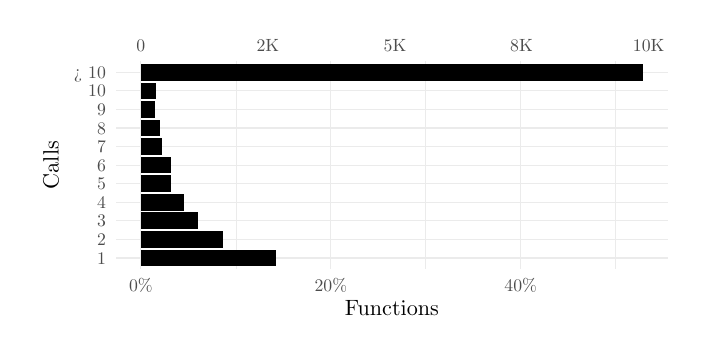
\begin{tikzpicture}[x=1pt,y=1pt]
\definecolor{fillColor}{RGB}{255,255,255}
\path[use as bounding box,fill=fillColor,fill opacity=0.00] (0,0) rectangle (238.49,108.41);
\begin{scope}
\path[clip] ( 31.86, 21.16) rectangle (231.38, 96.31);
\definecolor{drawColor}{gray}{0.92}

\path[draw=drawColor,line width= 0.2pt,line join=round] ( 75.23, 21.16) --
	( 75.23, 96.31);

\path[draw=drawColor,line width= 0.2pt,line join=round] (143.83, 21.16) --
	(143.83, 96.31);

\path[draw=drawColor,line width= 0.2pt,line join=round] (212.43, 21.16) --
	(212.43, 96.31);

\path[draw=drawColor,line width= 0.4pt,line join=round] ( 31.86, 25.19) --
	(231.38, 25.19);

\path[draw=drawColor,line width= 0.4pt,line join=round] ( 31.86, 31.90) --
	(231.38, 31.90);

\path[draw=drawColor,line width= 0.4pt,line join=round] ( 31.86, 38.61) --
	(231.38, 38.61);

\path[draw=drawColor,line width= 0.4pt,line join=round] ( 31.86, 45.32) --
	(231.38, 45.32);

\path[draw=drawColor,line width= 0.4pt,line join=round] ( 31.86, 52.03) --
	(231.38, 52.03);

\path[draw=drawColor,line width= 0.4pt,line join=round] ( 31.86, 58.73) --
	(231.38, 58.73);

\path[draw=drawColor,line width= 0.4pt,line join=round] ( 31.86, 65.44) --
	(231.38, 65.44);

\path[draw=drawColor,line width= 0.4pt,line join=round] ( 31.86, 72.15) --
	(231.38, 72.15);

\path[draw=drawColor,line width= 0.4pt,line join=round] ( 31.86, 78.86) --
	(231.38, 78.86);

\path[draw=drawColor,line width= 0.4pt,line join=round] ( 31.86, 85.57) --
	(231.38, 85.57);

\path[draw=drawColor,line width= 0.4pt,line join=round] ( 31.86, 92.28) --
	(231.38, 92.28);

\path[draw=drawColor,line width= 0.4pt,line join=round] ( 40.93, 21.16) --
	( 40.93, 96.31);

\path[draw=drawColor,line width= 0.4pt,line join=round] (109.53, 21.16) --
	(109.53, 96.31);

\path[draw=drawColor,line width= 0.4pt,line join=round] (178.13, 21.16) --
	(178.13, 96.31);
\definecolor{fillColor}{RGB}{0,0,0}

\path[fill=fillColor] ( 40.93, 89.26) rectangle (222.31, 95.30);

\path[fill=fillColor] ( 40.93, 22.17) rectangle ( 89.89, 28.21);

\path[fill=fillColor] ( 40.93, 28.88) rectangle ( 70.62, 34.92);

\path[fill=fillColor] ( 40.93, 35.59) rectangle ( 61.56, 41.63);

\path[fill=fillColor] ( 40.93, 42.30) rectangle ( 56.31, 48.34);

\path[fill=fillColor] ( 40.93, 55.72) rectangle ( 51.90, 61.75);

\path[fill=fillColor] ( 40.93, 49.01) rectangle ( 51.87, 55.04);

\path[fill=fillColor] ( 40.93, 62.43) rectangle ( 48.49, 68.46);

\path[fill=fillColor] ( 40.93, 69.13) rectangle ( 47.87, 75.17);

\path[fill=fillColor] ( 40.93, 82.55) rectangle ( 46.25, 88.59);

\path[fill=fillColor] ( 40.93, 75.84) rectangle ( 46.18, 81.88);
\end{scope}
\begin{scope}
\path[clip] (  0.00,  0.00) rectangle (238.49,108.41);
\definecolor{drawColor}{gray}{0.30}

\node[text=drawColor,anchor=base,inner sep=0pt, outer sep=0pt, scale=  0.64] at ( 40.85, 99.91) {0};

\node[text=drawColor,anchor=base,inner sep=0pt, outer sep=0pt, scale=  0.64] at ( 86.78, 99.91) {2K};

\node[text=drawColor,anchor=base,inner sep=0pt, outer sep=0pt, scale=  0.64] at (132.72, 99.91) {5K};

\node[text=drawColor,anchor=base,inner sep=0pt, outer sep=0pt, scale=  0.64] at (178.45, 99.91) {8K};

\node[text=drawColor,anchor=base,inner sep=0pt, outer sep=0pt, scale=  0.64] at (224.39, 99.91) {10K};
\end{scope}
\begin{scope}
\path[clip] (  0.00,  0.00) rectangle (238.49,108.41);
\definecolor{drawColor}{gray}{0.30}

\node[text=drawColor,anchor=base east,inner sep=0pt, outer sep=0pt, scale=  0.64] at ( 28.26, 22.98) {1};

\node[text=drawColor,anchor=base east,inner sep=0pt, outer sep=0pt, scale=  0.64] at ( 28.26, 29.69) {2};

\node[text=drawColor,anchor=base east,inner sep=0pt, outer sep=0pt, scale=  0.64] at ( 28.26, 36.40) {3};

\node[text=drawColor,anchor=base east,inner sep=0pt, outer sep=0pt, scale=  0.64] at ( 28.26, 43.11) {4};

\node[text=drawColor,anchor=base east,inner sep=0pt, outer sep=0pt, scale=  0.64] at ( 28.26, 49.82) {5};

\node[text=drawColor,anchor=base east,inner sep=0pt, outer sep=0pt, scale=  0.64] at ( 28.26, 56.53) {6};

\node[text=drawColor,anchor=base east,inner sep=0pt, outer sep=0pt, scale=  0.64] at ( 28.26, 63.24) {7};

\node[text=drawColor,anchor=base east,inner sep=0pt, outer sep=0pt, scale=  0.64] at ( 28.26, 69.95) {8};

\node[text=drawColor,anchor=base east,inner sep=0pt, outer sep=0pt, scale=  0.64] at ( 28.26, 76.66) {9};

\node[text=drawColor,anchor=base east,inner sep=0pt, outer sep=0pt, scale=  0.64] at ( 28.26, 83.37) {10};

\node[text=drawColor,anchor=base east,inner sep=0pt, outer sep=0pt, scale=  0.64] at ( 28.26, 90.08) {> 10};
\end{scope}
\begin{scope}
\path[clip] (  0.00,  0.00) rectangle (238.49,108.41);
\definecolor{drawColor}{gray}{0.30}

\node[text=drawColor,anchor=base,inner sep=0pt, outer sep=0pt, scale=  0.64] at ( 40.93, 13.15) {0{\%}};

\node[text=drawColor,anchor=base,inner sep=0pt, outer sep=0pt, scale=  0.64] at (109.53, 13.15) {20{\%}};

\node[text=drawColor,anchor=base,inner sep=0pt, outer sep=0pt, scale=  0.64] at (178.13, 13.15) {40{\%}};
\end{scope}
\begin{scope}
\path[clip] (  0.00,  0.00) rectangle (238.49,108.41);
\definecolor{drawColor}{RGB}{0,0,0}

\node[text=drawColor,anchor=base,inner sep=0pt, outer sep=0pt, scale=  0.80] at (131.62,  4.40) {Functions};
\end{scope}
\begin{scope}
\path[clip] (  0.00,  0.00) rectangle (238.49,108.41);
\definecolor{drawColor}{RGB}{0,0,0}

\node[text=drawColor,rotate= 90.00,anchor=base,inner sep=0pt, outer sep=0pt, scale=  0.80] at ( 11.20, 58.73) {Calls};
\end{scope}
\end{tikzpicture}

  \caption{Call Distribution}
  \label{fig:calldist}
\end{figure}

These functions have a total of 67,225 parameter positions.
Figure~\ref{fig:paramdist} shows the distribution of parameter positions.
3.0\% functions have 0 parameters, 22.4\% have 1, and 5.0\% have over
10. There are 4 functions with over 50 parameters that come from 3 packages. Of
those, \texttt{ggplot2::theme} has the highest, 95 parameters.

\begin{figure}[!h]
  \centering
  % Created by tikzDevice version 0.12.3.1 on 2021-06-03 17:14:19
% !TEX encoding = UTF-8 Unicode
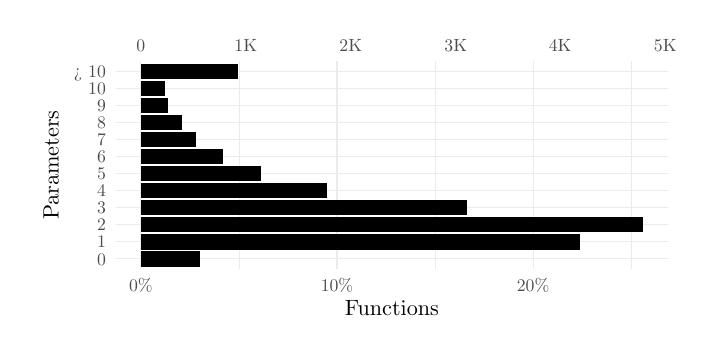
\begin{tikzpicture}[x=1pt,y=1pt]
\definecolor{fillColor}{RGB}{255,255,255}
\path[use as bounding box,fill=fillColor,fill opacity=0.00] (0,0) rectangle (238.49,108.41);
\begin{scope}
\path[clip] ( 31.86, 21.16) rectangle (231.38, 96.31);
\definecolor{drawColor}{gray}{0.92}

\path[draw=drawColor,line width= 0.2pt,line join=round] ( 76.35, 21.16) --
	( 76.35, 96.31);

\path[draw=drawColor,line width= 0.2pt,line join=round] (147.19, 21.16) --
	(147.19, 96.31);

\path[draw=drawColor,line width= 0.2pt,line join=round] (218.04, 21.16) --
	(218.04, 96.31);

\path[draw=drawColor,line width= 0.4pt,line join=round] ( 31.86, 24.86) --
	(231.38, 24.86);

\path[draw=drawColor,line width= 0.4pt,line join=round] ( 31.86, 31.02) --
	(231.38, 31.02);

\path[draw=drawColor,line width= 0.4pt,line join=round] ( 31.86, 37.18) --
	(231.38, 37.18);

\path[draw=drawColor,line width= 0.4pt,line join=round] ( 31.86, 43.34) --
	(231.38, 43.34);

\path[draw=drawColor,line width= 0.4pt,line join=round] ( 31.86, 49.50) --
	(231.38, 49.50);

\path[draw=drawColor,line width= 0.4pt,line join=round] ( 31.86, 55.66) --
	(231.38, 55.66);

\path[draw=drawColor,line width= 0.4pt,line join=round] ( 31.86, 61.81) --
	(231.38, 61.81);

\path[draw=drawColor,line width= 0.4pt,line join=round] ( 31.86, 67.97) --
	(231.38, 67.97);

\path[draw=drawColor,line width= 0.4pt,line join=round] ( 31.86, 74.13) --
	(231.38, 74.13);

\path[draw=drawColor,line width= 0.4pt,line join=round] ( 31.86, 80.29) --
	(231.38, 80.29);

\path[draw=drawColor,line width= 0.4pt,line join=round] ( 31.86, 86.45) --
	(231.38, 86.45);

\path[draw=drawColor,line width= 0.4pt,line join=round] ( 31.86, 92.61) --
	(231.38, 92.61);

\path[draw=drawColor,line width= 0.4pt,line join=round] ( 40.93, 21.16) --
	( 40.93, 96.31);

\path[draw=drawColor,line width= 0.4pt,line join=round] (111.77, 21.16) --
	(111.77, 96.31);

\path[draw=drawColor,line width= 0.4pt,line join=round] (182.62, 21.16) --
	(182.62, 96.31);
\definecolor{fillColor}{RGB}{0,0,0}

\path[fill=fillColor] ( 40.93, 89.84) rectangle ( 76.18, 95.38);

\path[fill=fillColor] ( 40.93, 22.09) rectangle ( 62.34, 27.63);

\path[fill=fillColor] ( 40.93, 28.25) rectangle (199.57, 33.79);

\path[fill=fillColor] ( 40.93, 83.68) rectangle ( 49.80, 89.22);

\path[fill=fillColor] ( 40.93, 34.41) rectangle (222.31, 39.95);

\path[fill=fillColor] ( 40.93, 40.56) rectangle (158.76, 46.11);

\path[fill=fillColor] ( 40.93, 46.72) rectangle (108.20, 52.27);

\path[fill=fillColor] ( 40.93, 52.88) rectangle ( 84.25, 58.43);

\path[fill=fillColor] ( 40.93, 59.04) rectangle ( 70.64, 64.59);

\path[fill=fillColor] ( 40.93, 65.20) rectangle ( 60.94, 70.75);

\path[fill=fillColor] ( 40.93, 71.36) rectangle ( 55.94, 76.91);

\path[fill=fillColor] ( 40.93, 77.52) rectangle ( 50.67, 83.06);
\end{scope}
\begin{scope}
\path[clip] (  0.00,  0.00) rectangle (238.49,108.41);
\definecolor{drawColor}{gray}{0.30}

\node[text=drawColor,anchor=base,inner sep=0pt, outer sep=0pt, scale=  0.64] at ( 40.85, 99.91) {0};

\node[text=drawColor,anchor=base,inner sep=0pt, outer sep=0pt, scale=  0.64] at ( 78.80, 99.91) {1K};

\node[text=drawColor,anchor=base,inner sep=0pt, outer sep=0pt, scale=  0.64] at (116.74, 99.91) {2K};

\node[text=drawColor,anchor=base,inner sep=0pt, outer sep=0pt, scale=  0.64] at (154.69, 99.91) {3K};

\node[text=drawColor,anchor=base,inner sep=0pt, outer sep=0pt, scale=  0.64] at (192.43, 99.91) {4K};

\node[text=drawColor,anchor=base,inner sep=0pt, outer sep=0pt, scale=  0.64] at (230.38, 99.91) {5K};
\end{scope}
\begin{scope}
\path[clip] (  0.00,  0.00) rectangle (238.49,108.41);
\definecolor{drawColor}{gray}{0.30}

\node[text=drawColor,anchor=base east,inner sep=0pt, outer sep=0pt, scale=  0.64] at ( 28.26, 22.65) {0};

\node[text=drawColor,anchor=base east,inner sep=0pt, outer sep=0pt, scale=  0.64] at ( 28.26, 28.81) {1};

\node[text=drawColor,anchor=base east,inner sep=0pt, outer sep=0pt, scale=  0.64] at ( 28.26, 34.97) {2};

\node[text=drawColor,anchor=base east,inner sep=0pt, outer sep=0pt, scale=  0.64] at ( 28.26, 41.13) {3};

\node[text=drawColor,anchor=base east,inner sep=0pt, outer sep=0pt, scale=  0.64] at ( 28.26, 47.29) {4};

\node[text=drawColor,anchor=base east,inner sep=0pt, outer sep=0pt, scale=  0.64] at ( 28.26, 53.45) {5};

\node[text=drawColor,anchor=base east,inner sep=0pt, outer sep=0pt, scale=  0.64] at ( 28.26, 59.61) {6};

\node[text=drawColor,anchor=base east,inner sep=0pt, outer sep=0pt, scale=  0.64] at ( 28.26, 65.77) {7};

\node[text=drawColor,anchor=base east,inner sep=0pt, outer sep=0pt, scale=  0.64] at ( 28.26, 71.93) {8};

\node[text=drawColor,anchor=base east,inner sep=0pt, outer sep=0pt, scale=  0.64] at ( 28.26, 78.09) {9};

\node[text=drawColor,anchor=base east,inner sep=0pt, outer sep=0pt, scale=  0.64] at ( 28.26, 84.25) {10};

\node[text=drawColor,anchor=base east,inner sep=0pt, outer sep=0pt, scale=  0.64] at ( 28.26, 90.41) {> 10};
\end{scope}
\begin{scope}
\path[clip] (  0.00,  0.00) rectangle (238.49,108.41);
\definecolor{drawColor}{gray}{0.30}

\node[text=drawColor,anchor=base,inner sep=0pt, outer sep=0pt, scale=  0.64] at ( 40.93, 13.15) {0{\%}};

\node[text=drawColor,anchor=base,inner sep=0pt, outer sep=0pt, scale=  0.64] at (111.77, 13.15) {10{\%}};

\node[text=drawColor,anchor=base,inner sep=0pt, outer sep=0pt, scale=  0.64] at (182.62, 13.15) {20{\%}};
\end{scope}
\begin{scope}
\path[clip] (  0.00,  0.00) rectangle (238.49,108.41);
\definecolor{drawColor}{RGB}{0,0,0}

\node[text=drawColor,anchor=base,inner sep=0pt, outer sep=0pt, scale=  0.80] at (131.62,  4.40) {Functions};
\end{scope}
\begin{scope}
\path[clip] (  0.00,  0.00) rectangle (238.49,108.41);
\definecolor{drawColor}{RGB}{0,0,0}

\node[text=drawColor,rotate= 90.00,anchor=base,inner sep=0pt, outer sep=0pt, scale=  0.80] at ( 11.20, 58.73) {Parameters};
\end{scope}
\end{tikzpicture}

  \caption{Parameter Distribution}
  \label{fig:paramdist}
\end{figure}

\section{Analyzing Environment Usage Patterns}

\subsection{Life Cycle of Environments}
In our corpus, we observe the creation of 1.2 B environments, which makes them
the second most widely allocated objects. Table~\ref{table:object_count_dist}
shows the distribution of R objects for comparison. Promises are the most widely
allocated objects, studied extensively by \citet{oopsla19b}. Vectors of logicals
and characters (string) are more frequently allocated compared to that of
integers, reals, and raw (bytes). Language objects, i.e, first-class
expressions, are used for metaprogramming. Lists are heterogeneous vectors.
Other objects such as S4, externalptr, etc. are rare.

\begin{table}
  \vspace{-3mm}
  \small
  \caption{Object Counts} \label{table:object_count_dist}
  \centering
  \begin{tabular}{lr}
    \toprule
    \textbf{Type}&\textbf{Count}\\
    \midrule
    Promise&3.0B\\
    Environment&1.2B\\
    Logical&1.1B\\
    Character&976.9M\\
    Language&506.6M\\
    Integer&482.0M\\
    \bottomrule
  \end{tabular}
  \begin{tabular}{lr}
    \toprule
    \textbf{Type}&\textbf{Count}\\
    \midrule
    List&168.2M\\
    Real&127.2M\\
    Closure&118.5M\\
    Symbol&74.3M\\
    Raw&50.1M\\
    Other&15.9M\\
    \bottomrule
  \end{tabular}
\end{table}

\paragraph{Where do environments come from?} The distribution of environments by
source is presented in Table~\ref{table:env_source_dist}. Environments are
implicitly created for scoping during function calls. This accounts for 99.4\%
of the environments observed in our corpus. Environments are also created by the
implementation for namespaces during package loading. This accounts for a meager
0.1\% of all the environments since these environments are bounded by the number
of packages loaded during program execution. 0.6\% of the environments are
created by miscellaneous sources.

\begin{table}
  \vspace{-3mm}
  \small
  \caption{Environment Source} \label{table:env_source_dist}
  \centering
  \begin{tabular}{l|rr}
    \toprule
    \textbf{Source}&\textbf{Count}&\textbf{Percentage}\\
    \midrule
    Call&1.2B&99.4\%\\
    Other&7.2M&0.6\%\\
    Package&672.5K&0.1\%\\
    \bottomrule
  \end{tabular}
\end{table}

\bibliography{bib/jv,bib/aviral}

\end{document}
